\chapter{Fundamental Notions from Calculus}
Welcome to the mathematical modeling class.  We'll start the class with a brief review of
the most basic ideas and notions from calculus.  If you have never taken a Calculus course
before then you should consider first taking a formal Calculus course before tackling this
class.  We only need a few of the main ideas for this class so what you'll find in this
chapter is necessarily brief.

\section{Sections from Active Calculus}
The \href{http://faculty.gvsu.edu/boelkinm/Home/AC/index.html}{Active Calculus Textbook}
is a wonderful online resource that stands in place of this chapter.  We will only discuss a
few select sections and you can find the relevant links below.  If you need further
reading to brush up on Calculus you should use the Active Calculus text.  
\begin{enumerate}
    \item Active Calculus Section 1.1: \href{https://activecalculus.org/single/sec-1-1-vel.html}{How do we
        measure velocity?}
    \item Active Calculus Section 1.2: \href{https://activecalculus.org/single/sec-1-2-lim.html}{The notion of a
        limit}
    \item Active Calculus Section 1.4
        \href{https://activecalculus.org/single/sec-1-4-derivative-fxn.html}{The
        Derivative Function}
    \item Active Calculus Section 2.1: 
        \href{https://activecalculus.org/single/sec-2-1-elem-rules.html}{Elementary
        derivative rules}
    \item Active Calculus Section 2.2: \href{https://activecalculus.org/single/sec-2-2-sin-cos.html}{The sine and cosine functions}
    \item Active Calculus Section 2.3: \href{https://activecalculus.org/single/sec-2-3-prod-quot.html}{The
        product and quotient rules}
    \item Active Calculus Section 2.4: \href{https://activecalculus.org/single/sec-2-5-chain.html}{The chain
        rule}
    \item Active Calculus Section 4.3: 
        \href{https://activecalculus.org/single/sec-4-3-definite-integral.html}{The
        definite integral}
    \item Active Calculus Section 4.4: \href{https://activecalculus.org/single/sec-4-4-FTC.html}{The Fundamental Theorem of Calculus}
\end{enumerate}


\section{Modeling Explorations with Calculus}
What remains in this chapter of these notes are several laboratory exercises meant to
support your review of Calculus and to introduce you to the basic notions of mathematical
modeling.  

\begin{lab}
Water is being drained from a hole near the bottom of a cylindrical tank. According to
Torrecelli's Law it can be shown that the rate at which the height $h$ of the water
changes is proportional to the square root of the height.  This can be written with
average rates of change as:
\begin{flalign}
    \text{average rate of change of the height} = \frac{\Delta h}{\Delta t} \approx K \cdot \sqrt{h} 
    \label{eqn:1.1.ex4}
\end{flalign}
where $K$ is a constant that depends on gravity as well as the size of the hole and the
shape of the tank.
\begin{center}
    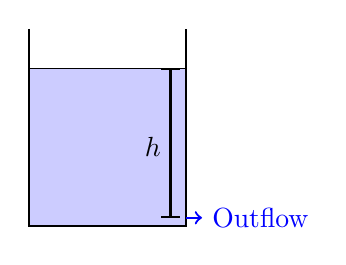
\begin{tikzpicture}
        \draw[fill=blue!20] (-1,2) -- (-1,0) -- (1,0) -- (1,2) -- cycle;
        \draw[thick, black] (-1,2.5) -- (-1,0) -- (1,0) -- (1,2.5);
        \draw[blue,thick, ->] (1,0.1) -- (1.2,0.1) node[anchor=west]{Outflow};
        \draw[thick, |-|] (0.8,0.1) -- (0.8,2);
        \draw (0.8,1) node[anchor=east]{$h$};
    \end{tikzpicture}
\end{center}

\begin{enumerate}
    \item[(a)] Using the video demonstration of Torrecelli's Law found here: \\
            \href{https://www.youtube.com/watch?v=gsNdsuQ1ZCo&app=desktop}{https://www.youtube.com/watch?v=gsNdsuQ1ZCo\&app=desktop}
            \\ and, using the pause button to your advantage, create a table of time vs.
            the height of the water in the container. Use as many data points as you feel
            necessary.
            \begin{center}
                \begin{tabular}{|c|c|}
                    \hline
                    Time (sec) & Height (cm) \\ \hline \hline
                    $\vdots$ & $\vdots$ \\
                    \hline
                \end{tabular}
            \end{center}
        \item[(b)] Use your data to estimate the value of $K$ in the experiment shown in the
            video. Be sure to include a discussion of units of $K$ and discuss which parts
            of this experiment are being described by $K$? \\ (Hint: Given equation
            \eqref{eqn:1.1.ex4}, what should a plot of $\sqrt{h}$ (on the $x$ axis) vs
            $\frac{\Delta h}{\Delta t}$ (on the $y$ axis) look like? How would you find
            $K$ from this plot?) 
        \item[(c)] Two more experiments were performed with different cylinders and different
            sized drain holes. Find the values of $K$ for each of these experiments, and
            from the data make comparisons between the sizes of the cylinders and the
            sizes of the holes for the three experiments.
            \begin{center}
                \begin{tabular}{|c|c|c|c|c|}
                    \hline
                    \multicolumn{2}{|c|}{Experiment \#1} & \hspace{0.2in} &
                    \multicolumn{2}{|c|}{Experiment \#2} \\ \hline 
                    Time (sec) & Height (cm) & & Time (sec) & Height (cm) \\ \hline \hline
                    0      & 35  & &  0     & 13  \\
                    8      & 30  & &  0.58  &  12\\
                    16     & 25  & &  1.35  &  11\\
                    25     & 20  & &  1.95  &  10\\
                    35.5   & 15  & &  2.85  &  9\\
                    48.7   & 10  & &  3.65  &  8\\
                    66.8   & 5   & &  4.55  &  7\\
                    &     & &  5.55  &  6\\
                    &     & &  6.55  &  5\\
                    &     & &  7.55  &  4\\
                    &     & &  8.55  &  3\\
                    &     & &  10.45 &  2\\
                    &     & &  13.45 &  1\\\hline
                \end{tabular}
            \end{center}
        \item[(d)] Discussion: What would happen if this experiment were run on a different,
            non-cylindrical, tank? Provide a detailed explanation.
    \end{enumerate}
\end{lab}

\begin{lab}
    A farmer with large land holdings has historically grown a wide variety of crops.
    With the price of ethanol fuel rising, he decides that it would be prudent to devote
    more and more of his acreage to producing corn.  As he grows more and more corn, he
    learns efficiencies that increase his yield per acre.  In the present year, he used
    7000 acres of his land to grow corn, and that land had an average yield of 170 bushels
    per acre.  At the current time, he plans to increase his number of acres devoted to
    growing corn at a rate of 600 acres/year, and he expects that right now his average
    yield is increasing at a rate of 8 bushels per acre per year.  Use this information to
    answer the following questions.
    \begin{enumerate}
        \item[(a)] Say that the present year is $t = 0$, that $A(t)$ denotes the number of acres the farmer devotes to growing corn in year $t$, $Y(t)$ represents the average yield in year $t$ (measured in bushels per acre), and $C(t)$ is the total number of bushels of corn the farmer produces.  What is the formula for $C(t)$ in terms of $A(t)$ and $Y(t)$?  Why?
        \item[(a)] What is the value of $C(0)$?  What does it measure?
        \item[(a)] Write an expression for $C'(t)$ in terms of $A(t)$, $A'(t)$, $Y(t)$, and $Y'(t)$.  Explain your thinking.
        \item[(a)] What is the value of $C'(0)$?  What does it measure?
        \item[(a)] Based on the given information and your work above, estimate the value of $C(1)$.	
        \item[(a)] Assume that the annual yield decreases every year by 8 bushels per acre.  Write
        expressions for $C(t)$ and $C'(t)$, find the approximate time and number of
        bushels when the total number of bushels is maximized, and discuss how the maximum
        value would change if the farmer were able to control the rate at which the yield
        decreased. Present your solution with thorough discussion and appropriate plots.
\end{enumerate}
\end{lab}

\begin{lab}
Let $f(v)$ be the gas consumption (in liters/km) of a car going at velocity $v$ (in km/hour). In other words, $f(v)$ tells you how many liters of gas the car uses to go one kilometer if it is traveling at $v$ kilometers per hour. In addition, suppose that $f(80)=0.05$ and $f'(80) = 0.0004$.
\begin{enumerate}
    \item[(a)] Let $g(v)$ be the distance the same car goes on one liter of gas at velocity $v$.  What is the relationship between $f(v)$ and $g(v)$? Hence find $g(80)$ and $g'(80)$.
    \item[(b)] Let $h(v)$ be the gas consumption in liters per hour of a car going at velocity $v$. In other words, $h(v)$ tells you how many liters of gas the car uses in one hour if it is going at velocity $v$.   What is the algebraic relationship between $h(v)$ and $f(v)$?  Hence find $h(80)$ and $h'(80)$.     
    \item[(c)] How would you explain the practical meaning of these function and derivative values to a driver who knows no calculus?  Include units on each of the function and derivative values you discuss in your response.  
\end{enumerate}

\end{lab}

\begin{lab}
The velocity (m/s) of an object dropped from a helicopter 1000 meters high is given in the
table below.  Use the velocity data to approximate the acceleration (m/s$^2$) and position
(m) data for the object at each of the given times.  Unfortunately the motion sensor broke
3 seconds into the experiment.  Extrapolate from the data to approximate the velocity and
acceleration when the object hit the ground.  Obviously there is drag on this object.
Make an argument to estimate when an object with 10\% more drag would hit the ground.
    
In your writeup of this problem:
    \begin{itemize}
        \item Be sure to give enough detail about the decisions and assumptions that you
            made.  
        \item Be sure to approximate the time that the object hit the ground in each
            instance.
        \item Be sure to thoroughly explain where calculus was (and wasn't) used in your
            solution.
    \end{itemize}

    \begin{center}
        \begin{tabular}{|c|c|}
            \hline
            Time (sec) & Velocity (meters/sec) \\ \hline \hline
            $0.0  $&$0$\\
            $0.2$&$-1.96$\\
            $0.4$&$-3.89$\\
            $0.6$&$-5.70$\\
            $0.8$&$-7.33$\\
            $1.0  $&$-8.76$\\
            $1.2$&$-9.95$\\
            $1.4$&$-10.92$\\
            $1.6$&$-11.69$\\
            $1.8$&$-12.29$\\
            $2.0  $&$-12.74$\\
            $2.2$&$-13.08$\\
            $2.4$&$-13.33$\\
            $2.6$&$-13.52$\\
            $2.8$&$-13.65$\\
            $3.0  $&$-13.75$\\\hline
        \end{tabular}
    \end{center}
\end{lab}


\begin{lab}
   Consider the following letter:
\begin{flushright}
    11 Patinkin Way \\
    First National Park of Drachma \\
\end{flushright}
\begin{flushleft}
    Mathematics Students \\
    Carroll College \\
    Helena, MT, USA
\end{flushleft}

\noindent Dear Calculus Students:

Things have finally quieted down around Drachma since the Prince was kicked out of office.
The good news is that I've managed to find a government job as the head of the First
National Park of Drachma.  The bad news is that most of the Park consists of a Fire Swamp
(google {\it fire swamp} if you need to).  When I went looking for help with our long
range planning, your enterprising and resourceful professor naturally referred me to you.

We have two species that have me worried about the future of the Park: the indigenous ROUS
(rodents of unusual size) and the brown tree snake which entered the Park about 50 years
ago as a stowaway on the Dread Pirate Roberts' ship.  Fortunately, ROUS's eat brown tree snakes.
Unfortunately, brown tree snakes reproduce very rapidly.

My predecessor at the Park was a meticulous census taker, so I have records of approximate
populations for each species for a 30 year period (see Table \ref{tab:pop_table}).

\begin{table}[h!]
    \begin{center}
        \begin{tabular}{|c|c|c|}
            \hline
            Year & Brown Tree Snakes & ROUS's \\ \hline \hline
            1982 & 15,300   & 415       \\
            1984 & 9,890    & 910       \\
            1986 & 2,860    & 950       \\
            1988 & 3,340    & 525       \\
            1990 & 9,340    & 250       \\
            1992 & 12,290   & 460       \\
            1994 & 9,050    & 830       \\
            1996 & 4,840    & 855       \\
            1998 & 5,130    & 545       \\
            2000 & 8,720    & 340       \\
            2002 & 10,490   & 500       \\
            2004 & 8,550    & 770       \\
            2006 & 6,030    & 790       \\
            2008 & 6,200    & 560       \\
            2010 & 8,350    & 410       \\
            2012 & 9,410    & 525       \\
            \hline
        \end{tabular}
        \caption{Populations by year since 1982.}
        \label{tab:pop_table}
    \end{center}
\end{table}

It looks like the populations are following some sort of pattern, but I'm not sure what it
is.  My real problem is that when either population gets very large, I will need
additional employees to make sure that both species stay within the park and don't escape
in the neighboring farmland.  This is where I need your expert help. Specifically, I need
a prediction for how large the populations will be in each of the next 20 years.  I also
need an estimate of the rate at which each of the populations are changing with
time\footnote{I'm thinking that a plot with time on the $x$-axis and average rate of
change on the $y$-axis might be very informative}. When the rates of change of the
populations are largest the local witch doctors head into the woods to raid the snake
nests and ROUS borrows for potion ingredients. 

I believe that the populations are fluctuating less and less, and may eventually
stabilize. I would like your expert opinion on whether or not the populations do stabilize,
and if they do, I need to know how long it will take and what the eventual populations
will be.

Once the populations stop fluctuating so drastically, we will be able to dramatically
improve access to the Park by offering summer camps, establishing permanent camp grounds,
and perhaps even adding a log ride.  There are still some flame-retardant issues
to be worked out and the 6-fingered man is terribly afraid of the log ride idea.  This
should all be possible when the ROUS population is fluctuating by less than 75 per year
and the brown tree snake population is fluctuating by less than 500 per year.  I need your
expert recommendation on when this will occur.

I have a meeting with the Budget Advisory Committee in 8 days to propose our budget
for the next two decades, so I would greatly appreciate your group's report in 1 week.

\vspace{0.2in}
\noindent Gratefully yours, \\
Amigo Flamboya

\vspace{0.5in}
\noindent {\bf Notes from your professor:} 
\begin{itemize}
    \item Work in groups of 2 or 3, but don't be afraid to bounce ideas off of other
        groups.
    \item To see the general trend of the populations, I would suggest plotting the points
        for each population separately (maybe in Excel), with time on the horizontal axis
        and population on the vertical axis. It may make things a bit easier if you let
        $t=0$ be 1982.
    \item Hint: Once you plot the populations, what two major types of functions do you
        see controlling the behavior?  You can fit the function by estimating things like
        the period (or frequency), the equilibrium value, and the function that controls
        the amplitude.  
%     \item Use the ideas from Lab 1 to help you figure out what the functions are. \\ Hint:
%         For each population the function is approximately trigonometric with an
%         exponentially decreasing amplitude. You likely won't be able to match the data
%         exactly, but you should be able to get close.
    \item Be sure to respond to Amigo Flamboya with an appropriate technical report.  He
        understands mathematics quite well so don't be afraid to include all necessary
        detail (explanations, plots, functions, etc) in your report. Make sure that you
        answer every question.
\end{itemize}
\end{lab}
